%Update 2020: Meritxell
\documentclass[11pt,a4paper]{article}
% Packages
\usepackage[latin1]{inputenc}
%\usepackage[english]{babel}
\usepackage{graphicx}
\usepackage{amsmath}
\usepackage{hyperref}
\usepackage{verbatim}
\usepackage{listings}
\usepackage{xcolor}
\usepackage{float}
\usepackage{chngcntr}
\usepackage[framed,numbered,autolinebreaks,useliterate]{mcode}
\usepackage{url}
\usepackage{afterpage}


%Subsection of the form 1.a instead of 1.1
\counterwithin*{subsection}{section}
\renewcommand{\thesubsection}{\thesection.\alph{subsection}}

%Add a blank page
\newcommand\blankpage{%
    \null
    \newpage}


\definecolor{codegreen}{rgb}{0,0.6,0}
\definecolor{codegray}{rgb}{0.5,0.5,0.5}
\definecolor{codepurple}{rgb}{0.58,0,0.82}
\definecolor{backcolour}{rgb}{0.95,0.95,0.92}

\lstdefinestyle{mystyle}{
    backgroundcolor=\color{backcolour},   
    commentstyle=\color{codegreen},
    keywordstyle=\color{magenta},
    numberstyle=\tiny\color{codegray},
    %identifierstyle=\color{blue},
    stringstyle=\color{codepurple},
    basicstyle=\ttfamily\footnotesize,
    breakatwhitespace=false,         
    breaklines=true,                 
    captionpos=b,                    
    keepspaces=true,                 
    numbers=left,                    
    numbersep=5pt,                  
    showspaces=false,                
    showstringspaces=false,
    showtabs=false,                  
    tabsize=2
}

\lstset{style=mystyle}

%% Format de la page
\pagestyle{plain}
%\setlength{\hoffset}{-0.4mm}
%\setlength{\voffset}{-1.4mm}%{-5.4mm}
\setlength{\oddsidemargin}{0mm}
%\setlength{\topmargin}{0mm}
%\setlength{\headheight}{0mm}
%\setlength{\headsep}{0mm}
\setlength{\textheight}{225mm}
\setlength{\textwidth}{160mm}
\newlength{\thickness} \setlength{\thickness}{0.2mm}
\setlength{\parindent}{0cm}
%\setlength{\parskip}{4pt}

\title{Project_1}
\author{raphael.mirallie }
\date{December 2020}

\begin{document}
\noindent \parbox[b]{12 cm}{
  \small
{\bf EPFL, Swiss Federal Institute of Technology in Lausanne} \\
{\bf SMA}

\bigskip

{\bf Numerical methods for conservation Laws}\\
{\bf Dr. Deep Ray}\\
{\bf Fall 2020}

} \hfill 
\includegraphics[width=4cm]{epfl_logo.jpg}

\noindent\hrulefill\\
\centerline{\large \bf One-dimensional shallow water equation using MUSCL reconstruction}\vspace{2ex}
\centerline{\bf Project 2}
\centerline{\bf  Axel Dinh Van Chi, Rapha\"el Miralli\'e}

\graphicspath{ {pictures/} }

%------------------------------------------------------------------------

\section{Question 1}

\subsection{}
The choice of M was done heuristically. After some testing, M = 100 seems to be a good compromise.

\subsection{}
Plot of the solutions and the error for the LF scheme can be found in Figure \ref{fig:LF_IC_1} and in Figure \ref{fig:LF_IC_1_error} respectively.
Plot of the solutions and the error for the Roe scheme can be found in Figure \ref{fig:Roe_IC_1} and in Figure \ref{fig:Roe_IC_1_error} respectively.

%------------------------------------------------------------------------

\section{Question 2}

\subsection{}
Plot of the solutions for the LF scheme can be found in Figure \ref{fig:LF_IC_2} and in Figure \ref{fig:LF_IC_3} for IC (6) and (7) respectively.

Plot of the solutions for the LF scheme can be found in Figure \ref{fig:Roe_IC_2} and in Figure \ref{fig:Roe_IC_3} for IC (6) and (7) respectively.


\subsection{}
\subsection{}

Plot of the errors for the LF scheme can be found in Figure \ref{fig:LF_IC_2_error} and in Figure \ref{fig:LF_IC_3_error} for IC (6) and (7) respectively.

Plot of the errors for the LF scheme can be found in Figure \ref{fig:Roe_IC_2_error} and in Figure \ref{fig:Roe_IC_3_error} for IC (6) and (7) respectively.

%------------------------------------------------------------------------

\section{Question 3}

\subsection{}
Plot of the solutions for the LF and for the Roe scheme can be found in Figure \ref{fig:FL_IC_4} and in Figure \ref{fig:Roe_IC_4} respectively.

\subsection{}

It does. 

%------------------------------------------------------------------------
\newpage
\section{Figures}

%1_b
\begin{figure}[!htb]
    \centering
    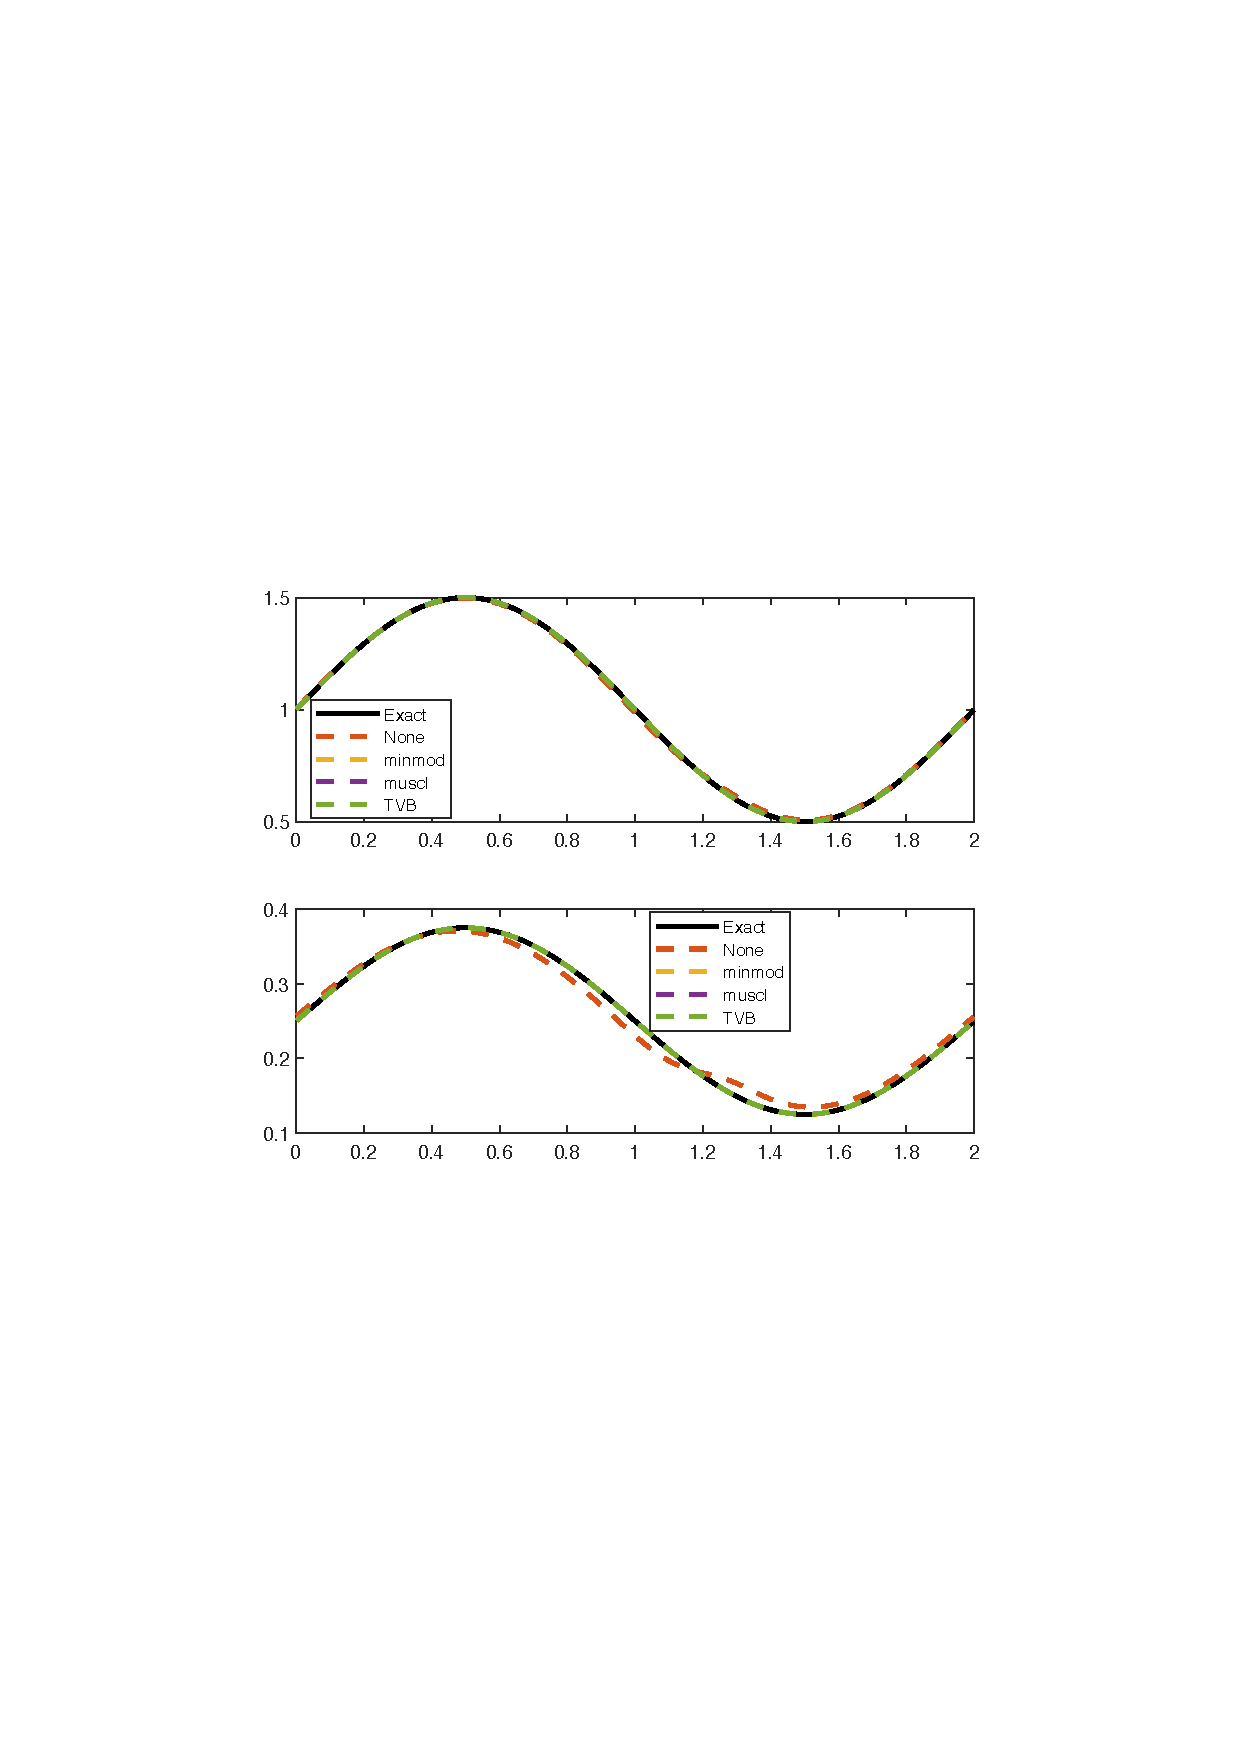
\includegraphics[width=11cm]{2_1_b_LF.pdf}
    \caption{LF method at T=2, 500 cells, IC (2)}
    \label{fig:LF_IC_1}
\end{figure}

\begin{figure}[!htb]
    \centering
    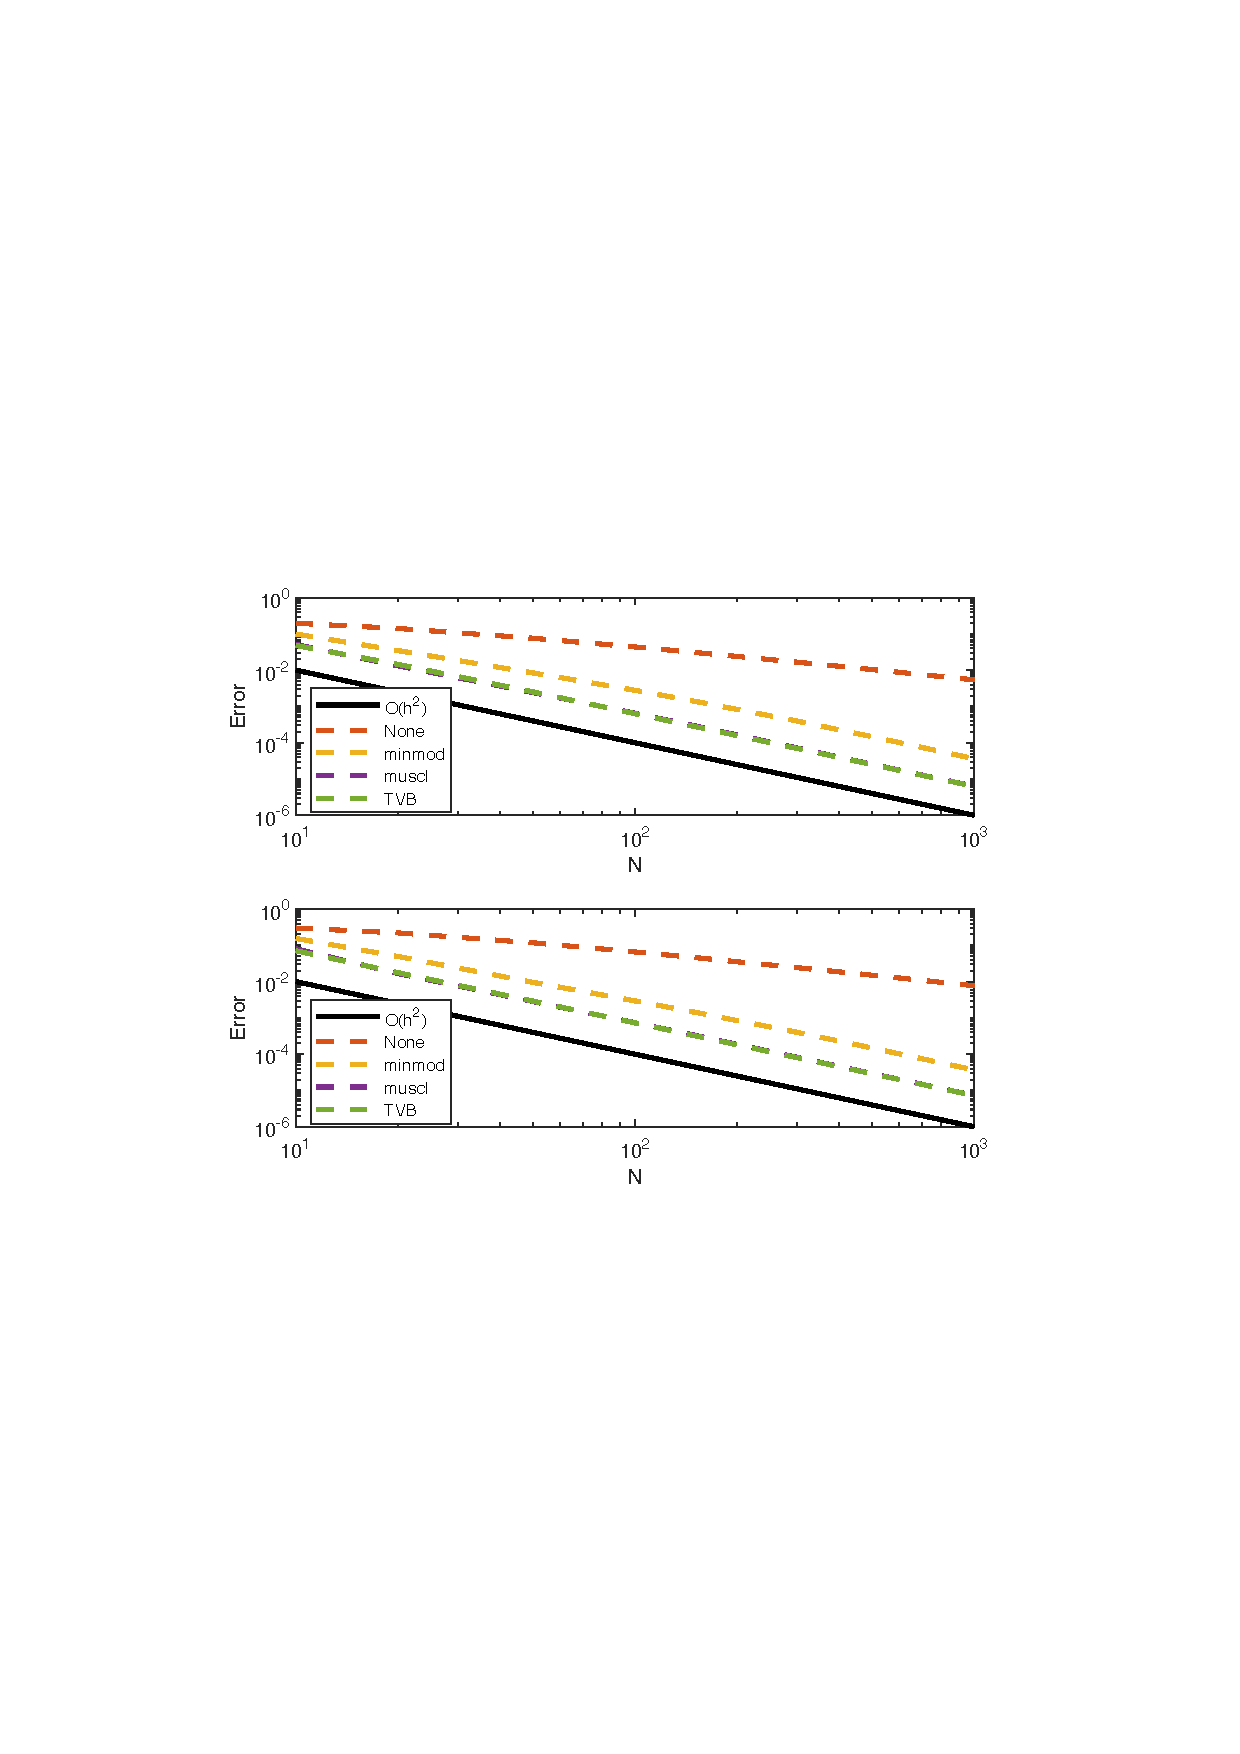
\includegraphics[width=11cm]{2_1_b_LF_error.pdf}
    \caption{LF method errors, 500 cells, IC (2)}
    \label{fig:LF_IC_1_error}
\end{figure}

\begin{figure}[!htb]
    \centering
    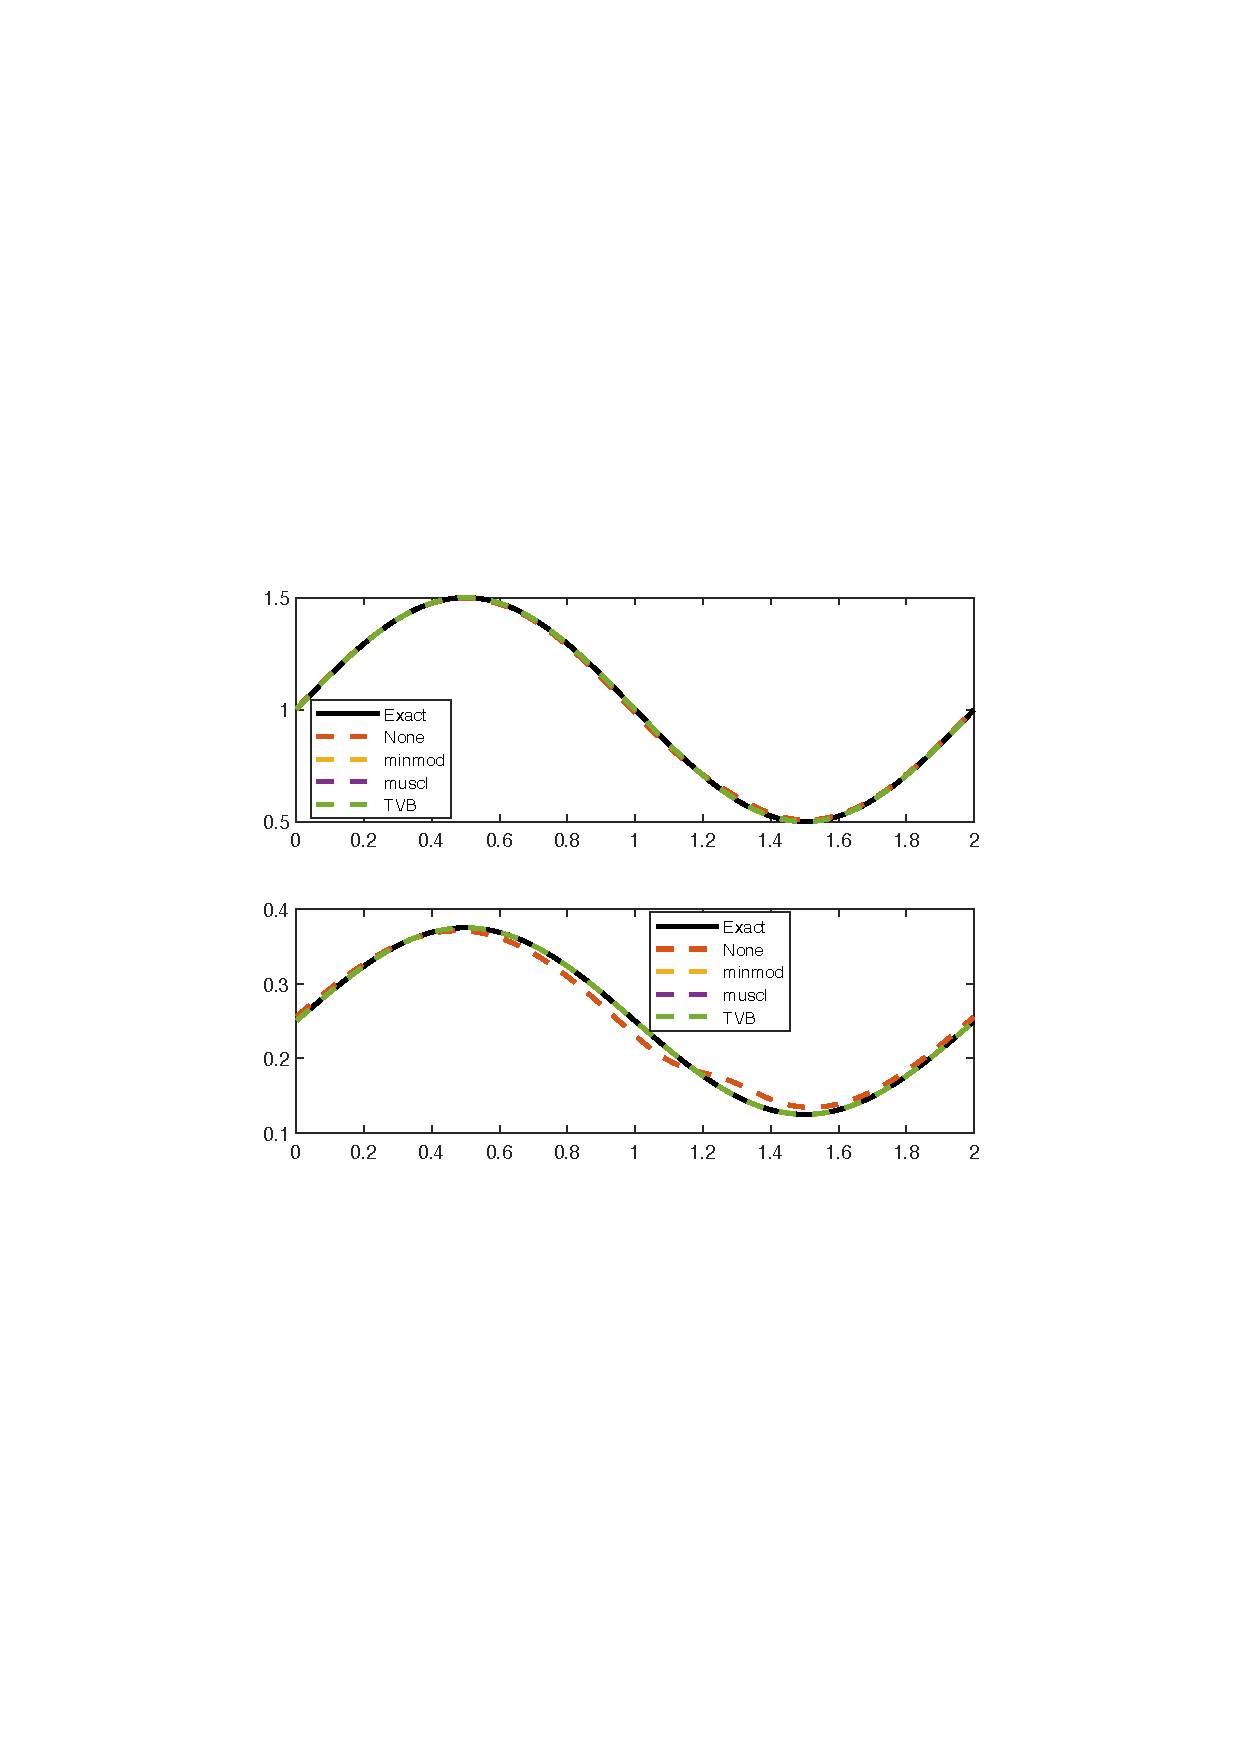
\includegraphics[width=11cm]{2_1_b_Roe.pdf}
    \caption{LF method at T=2, 500 cells, IC (2)}
    \label{fig:Roe_IC_1}
\end{figure}

\begin{figure}[!htb]
    \centering
    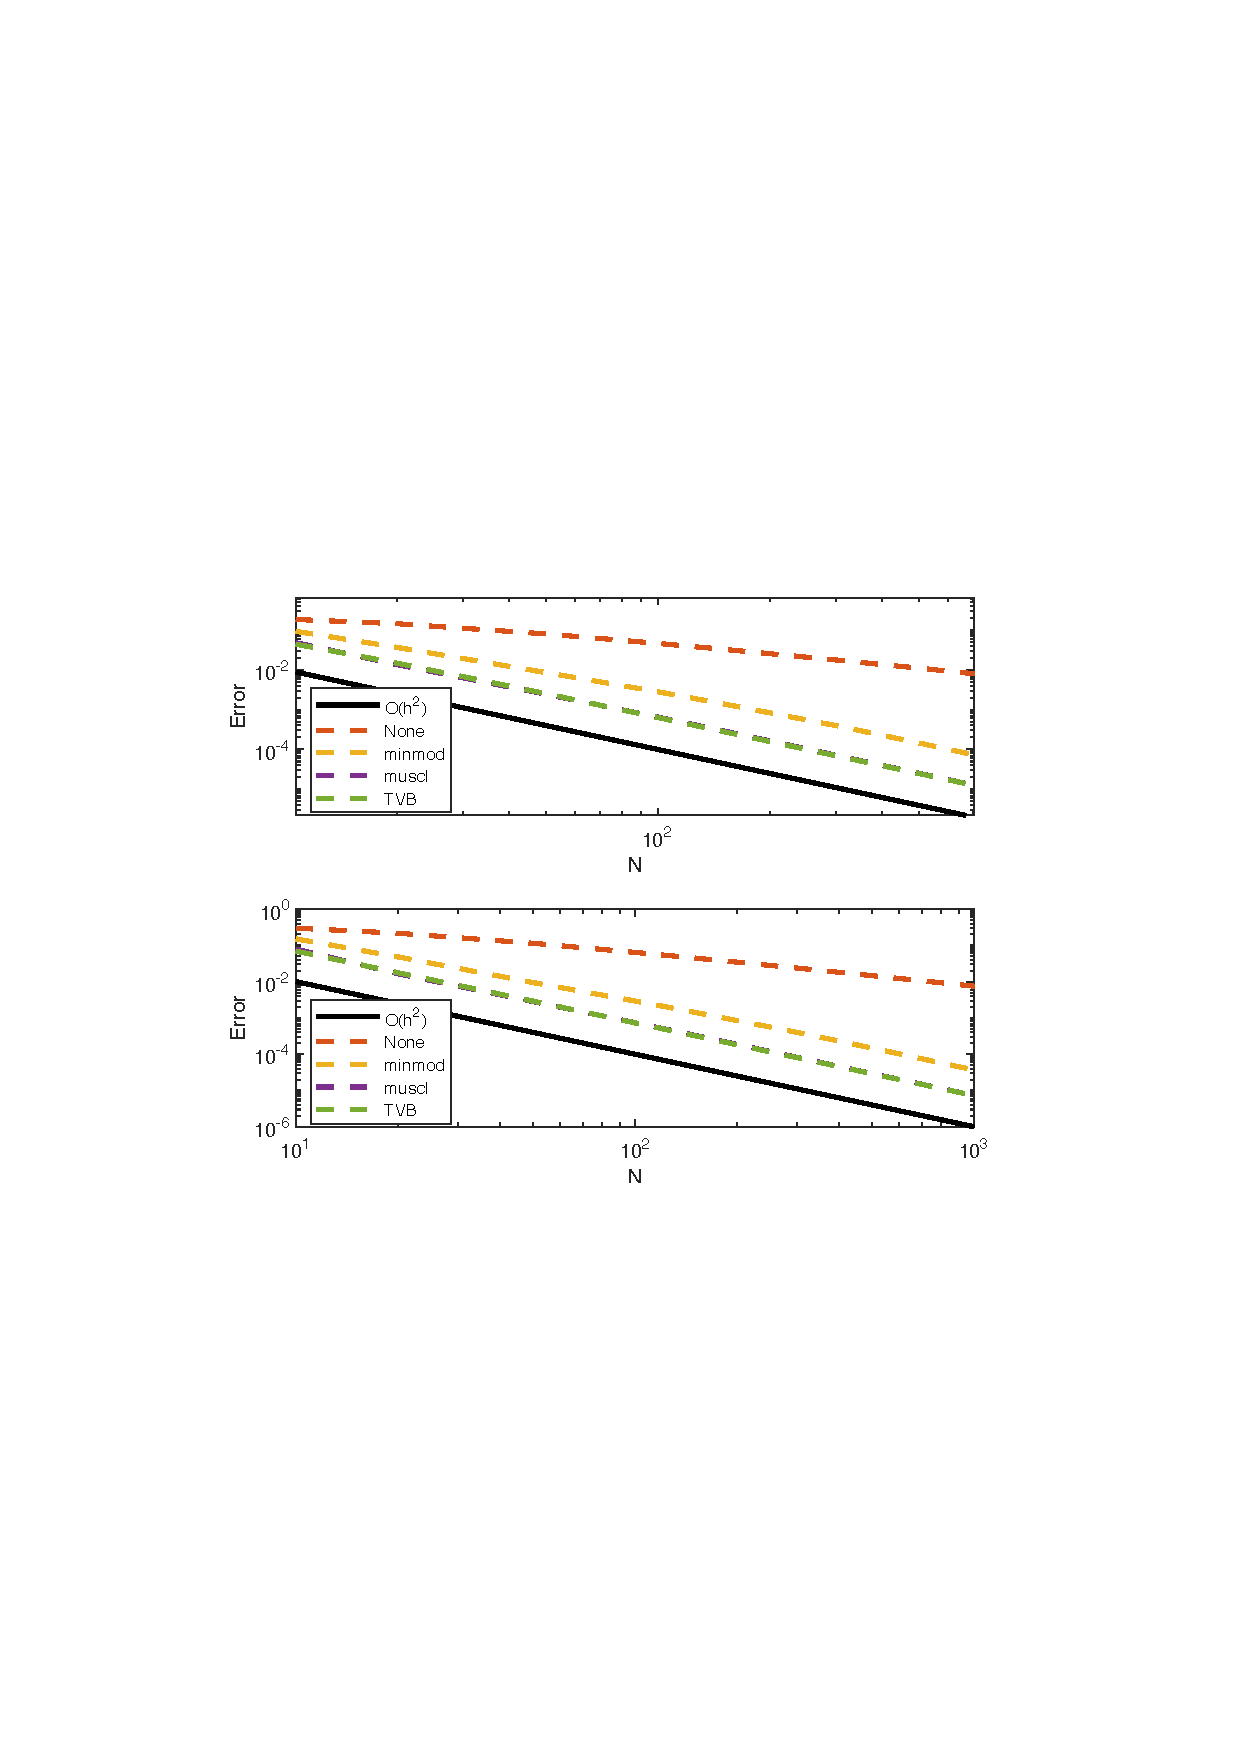
\includegraphics[width=11cm]{2_1_b_Roe_error.pdf}
    \caption{LF method errors, 500 cells, IC (2)}
    \label{fig:Roe_IC_1_error}
\end{figure}

%2_a / 2_c
\begin{figure}[!htb]
    \centering
    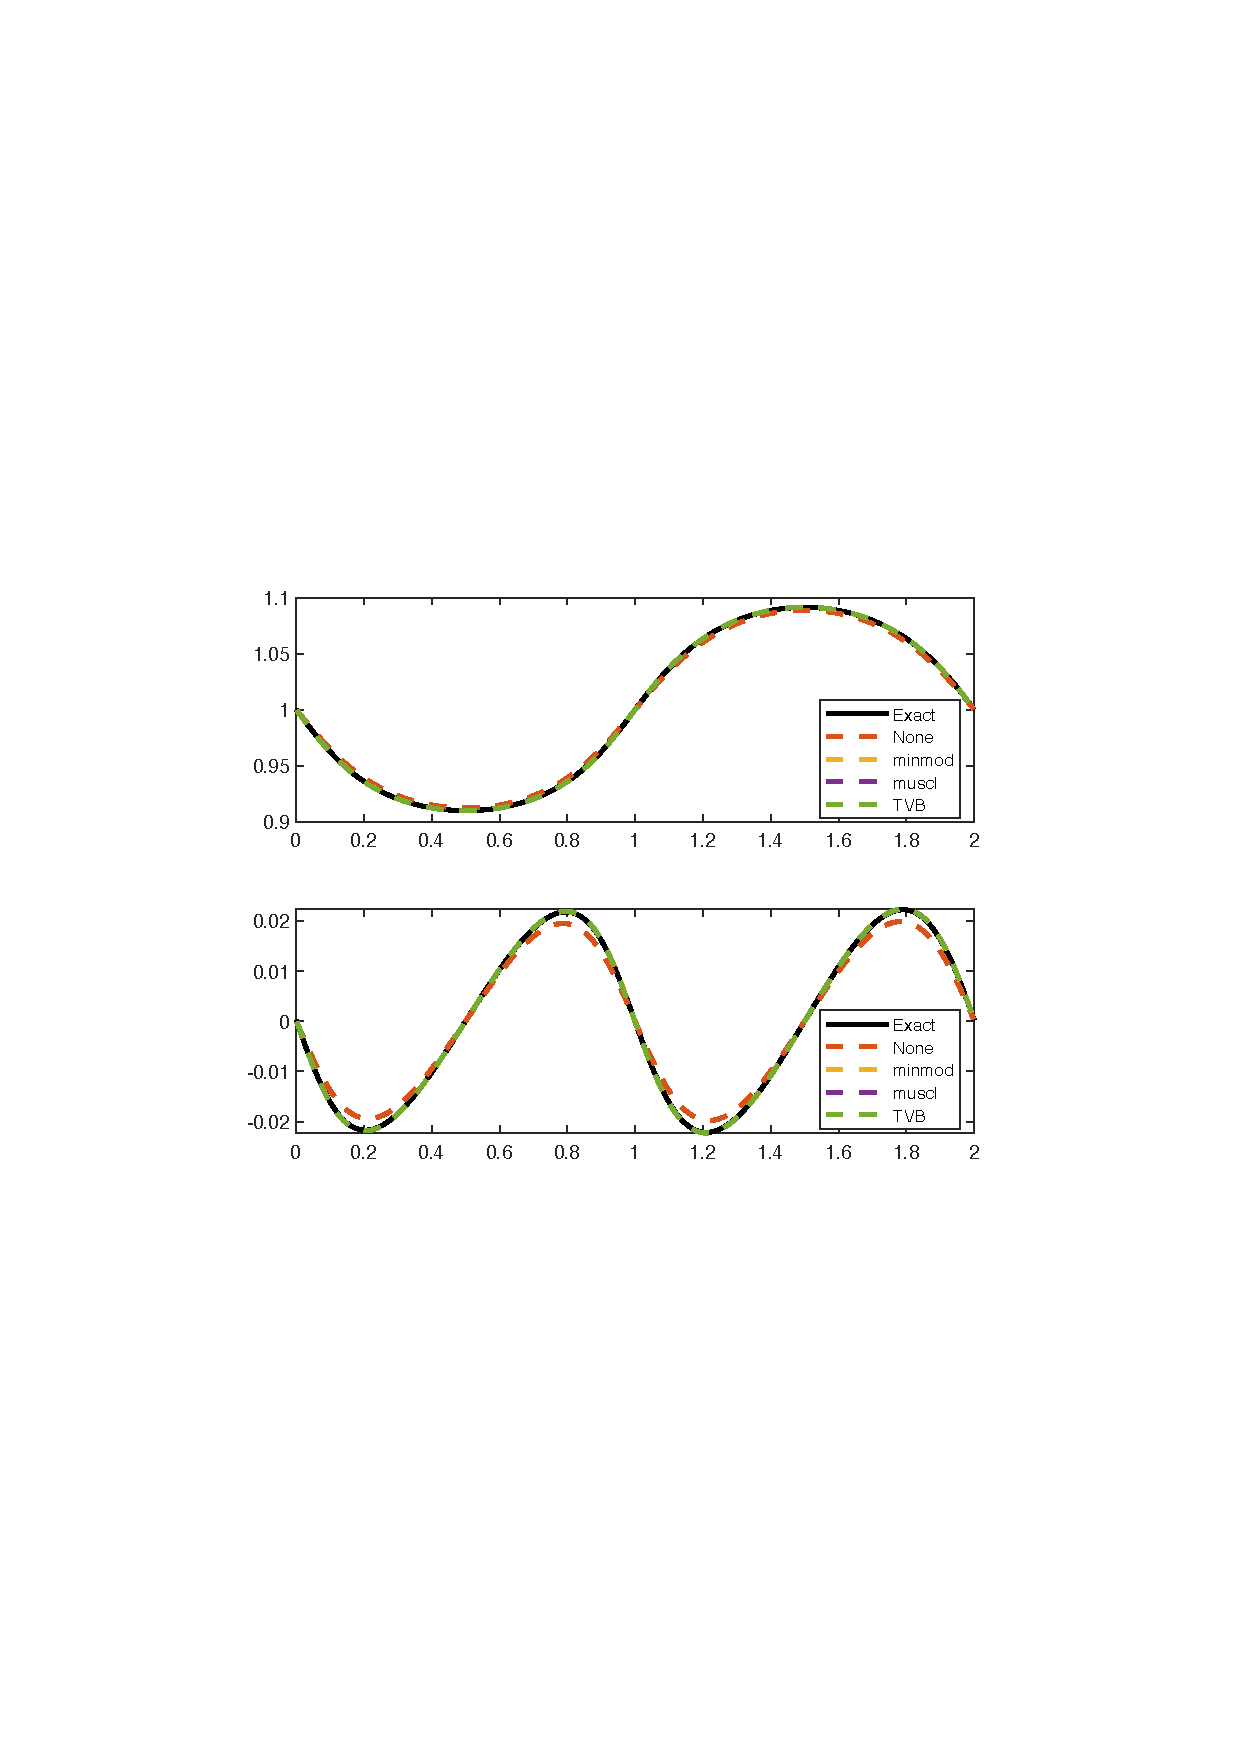
\includegraphics[width=11cm]{2_2_a_IC_2_LF.pdf}
    \caption{LF method errors, 500 cells, IC (6)}
    \label{fig:LF_IC_2}
\end{figure}

\begin{figure}[!htb]
    \centering
    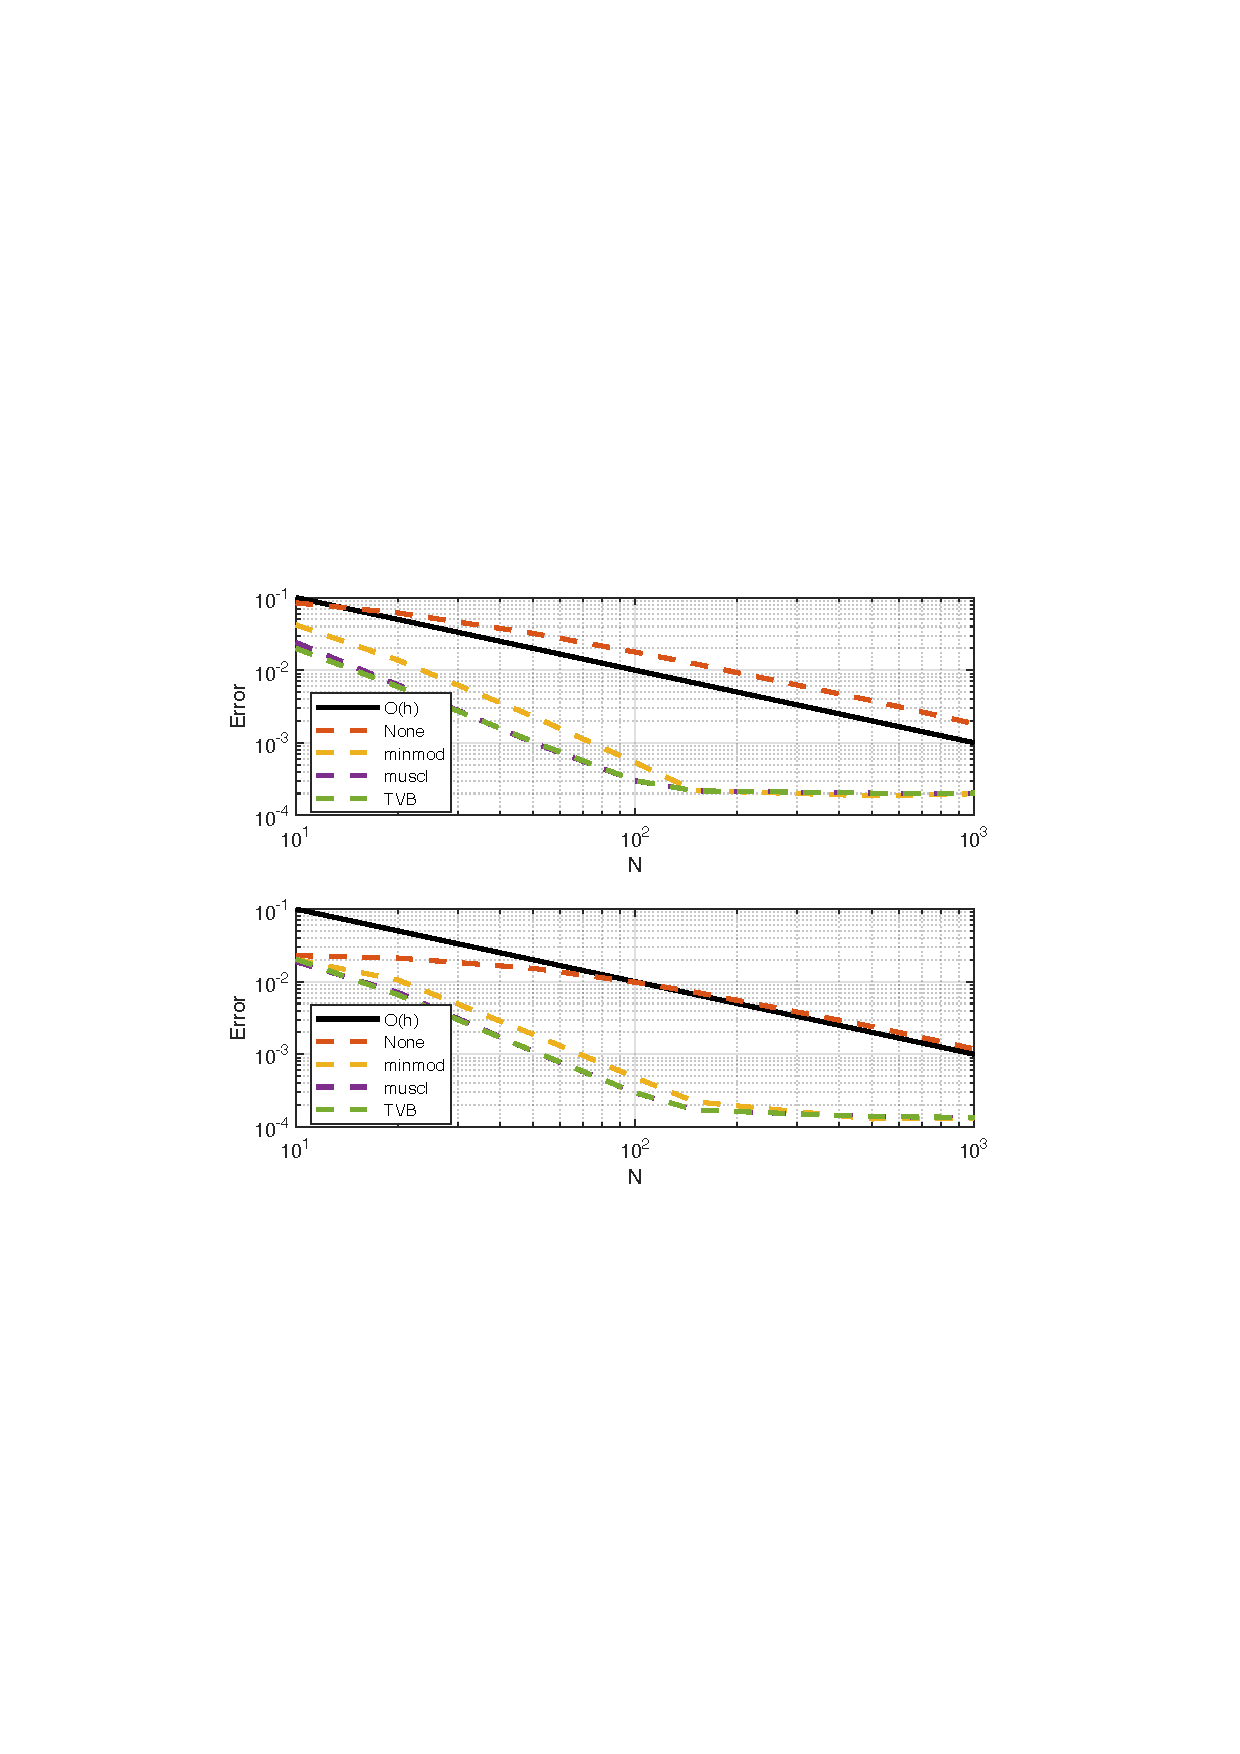
\includegraphics[width=11cm]{2_2_c_IC_2_LF.pdf}
    \caption{LF method at T=2, 500 cells, IC (6)}
    \label{fig:LF_IC_2_error}
\end{figure}

\begin{figure}[!htb]
    \centering
    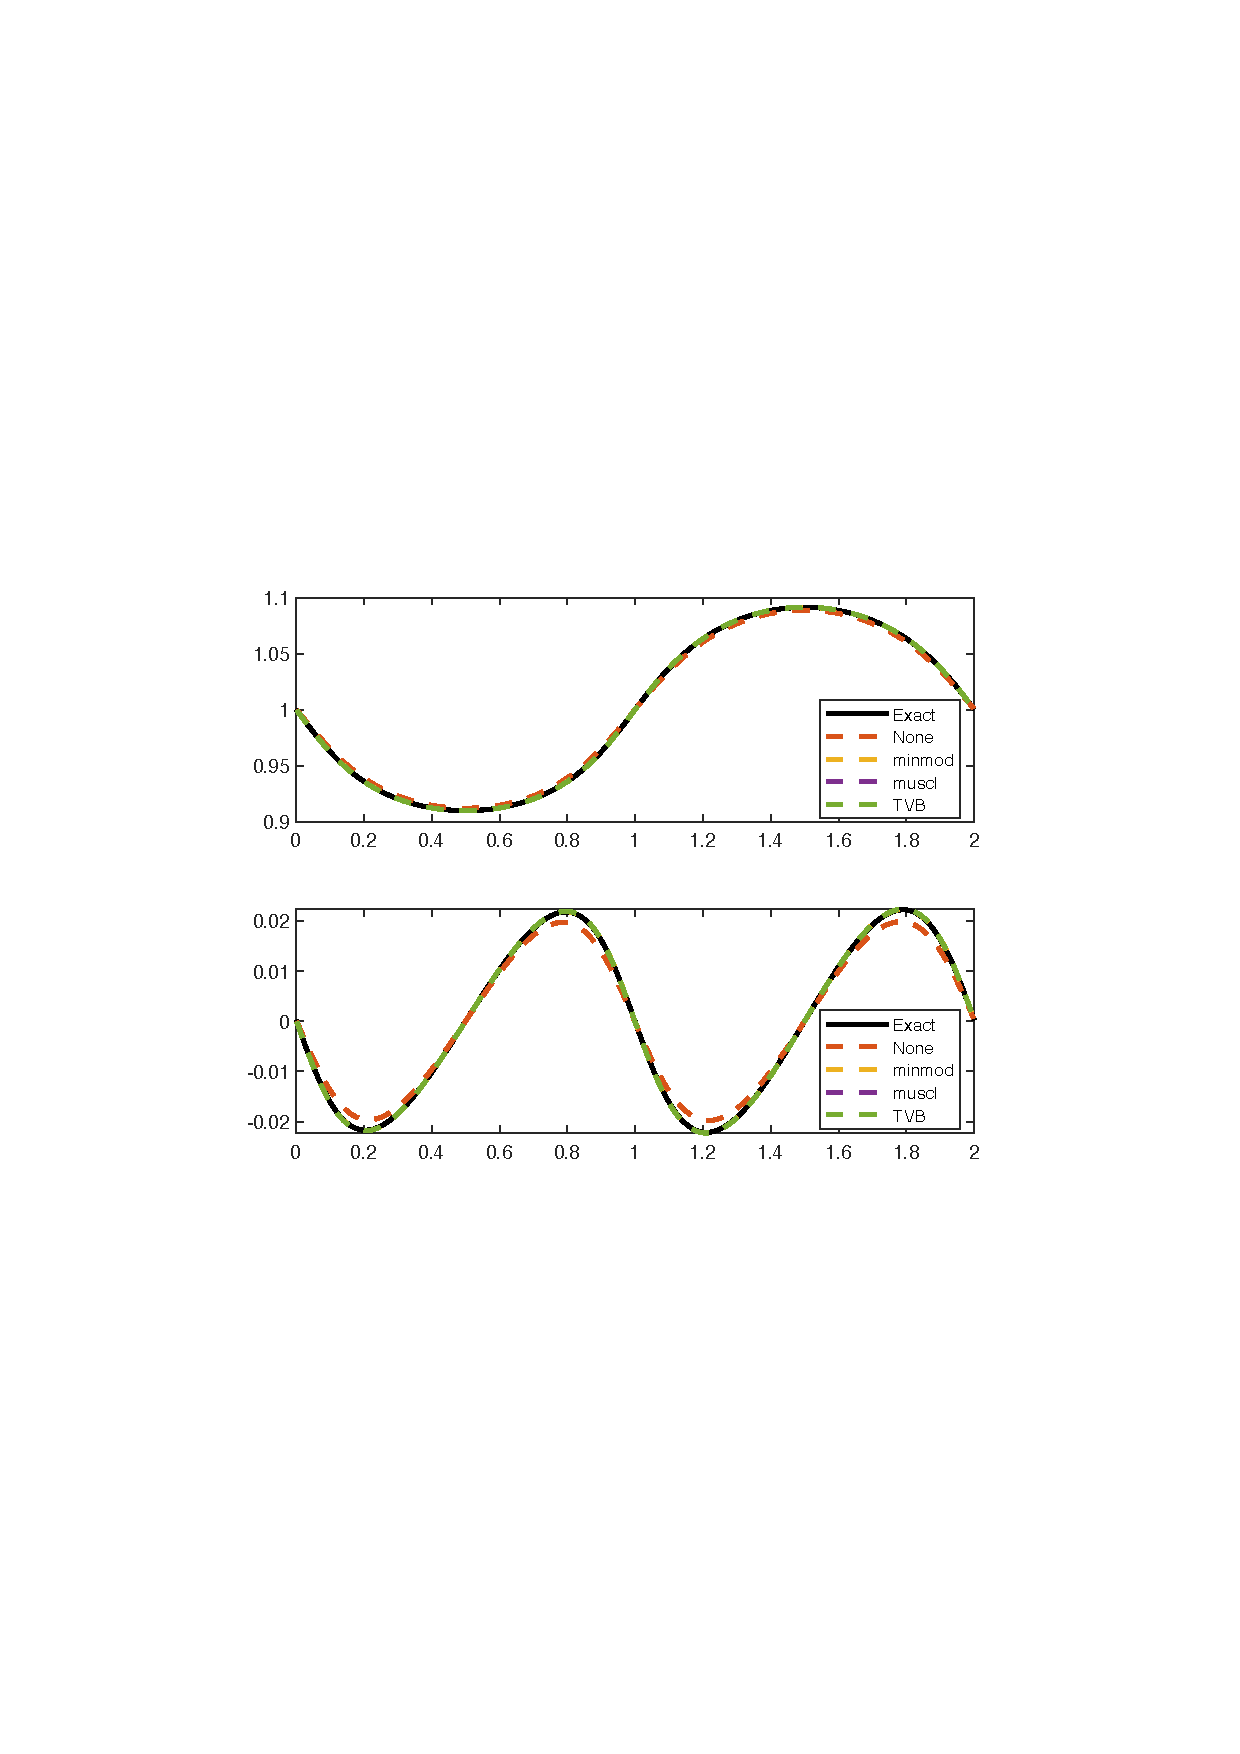
\includegraphics[width=11cm]{2_2_a_IC_2_Roe.pdf}
    \caption{Roe method errors, 500 cells, IC (6)}
    \label{fig:Roe_IC_2}
\end{figure}

\begin{figure}[!htb]
    \centering
    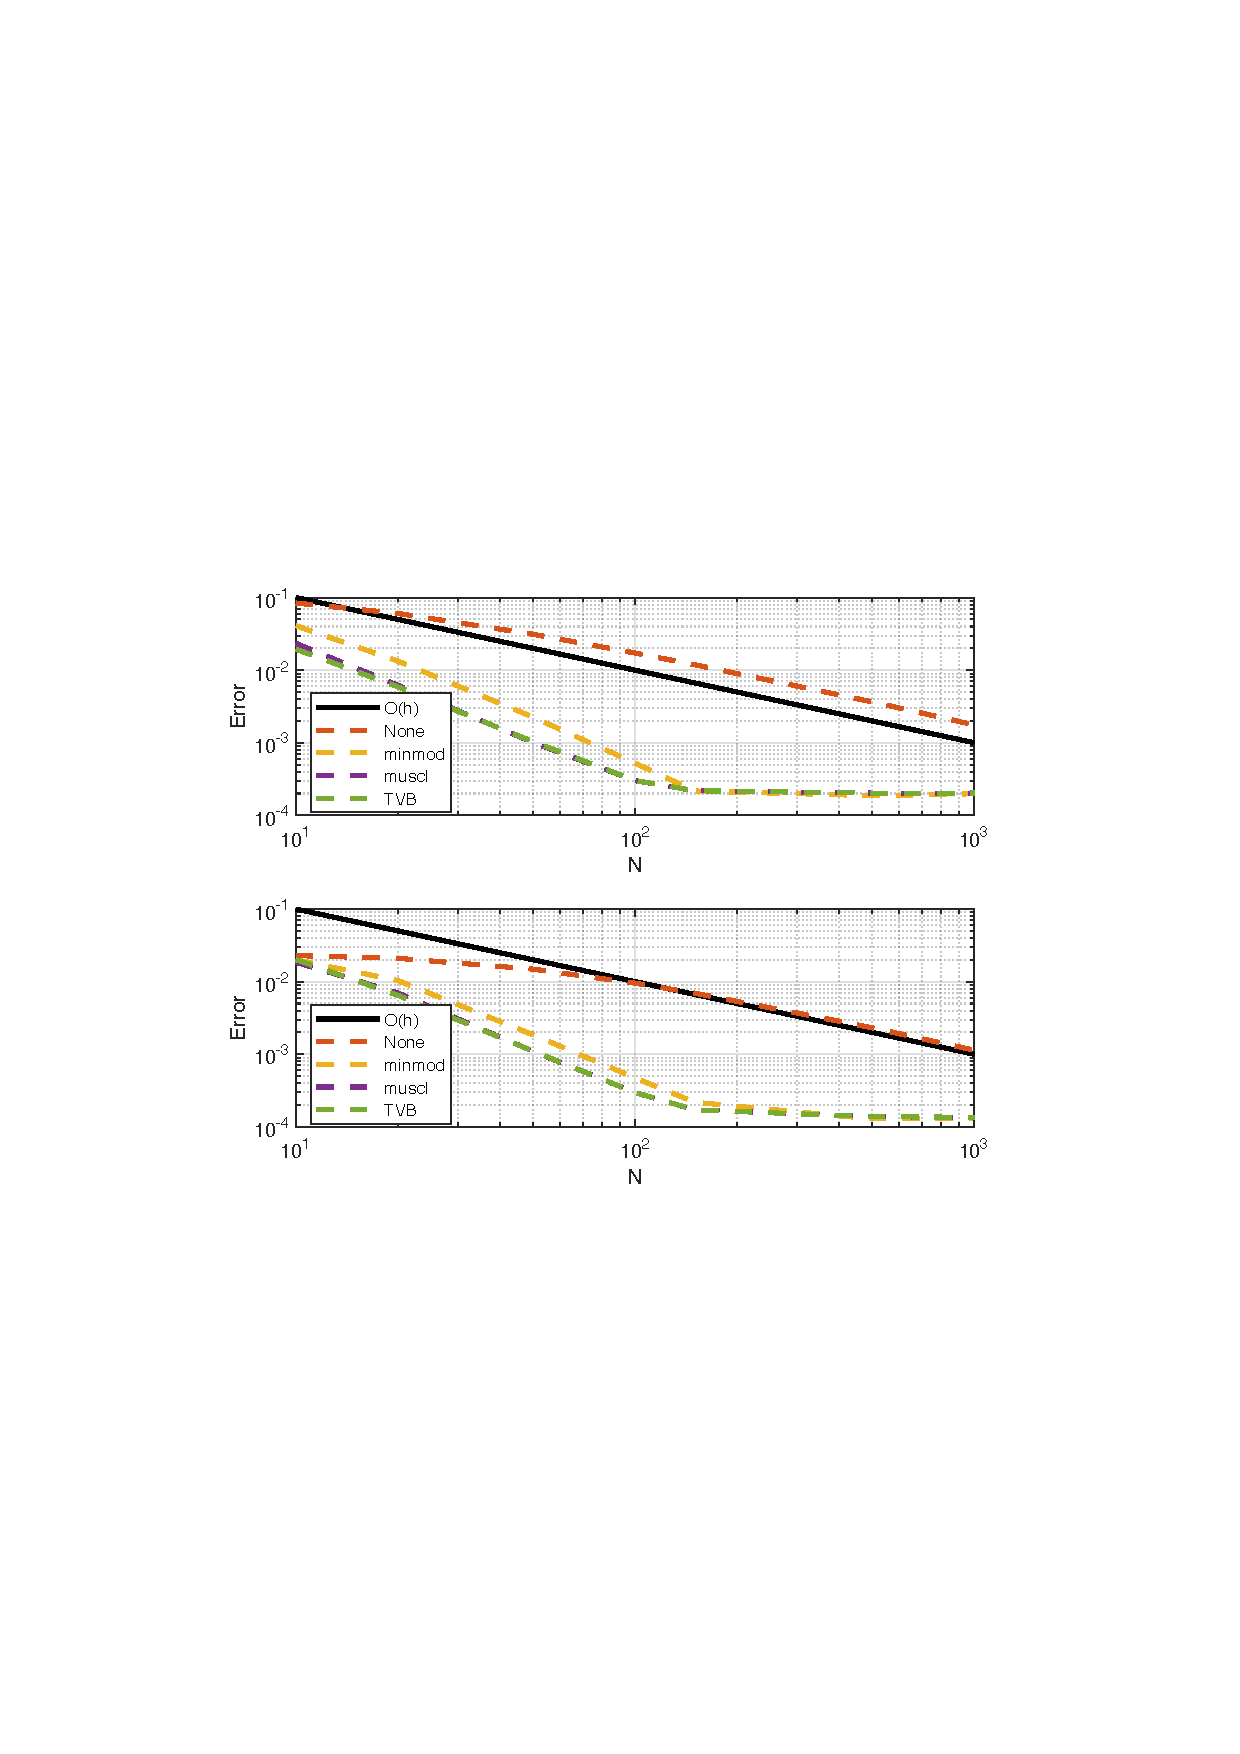
\includegraphics[width=11cm]{2_2_c_IC_2_Roe.pdf}
    \caption{Roe method at T=2, 500 cells, IC (6)}
    \label{fig:Roe_IC_2_error}
\end{figure}

\begin{figure}[!htb]
    \centering
    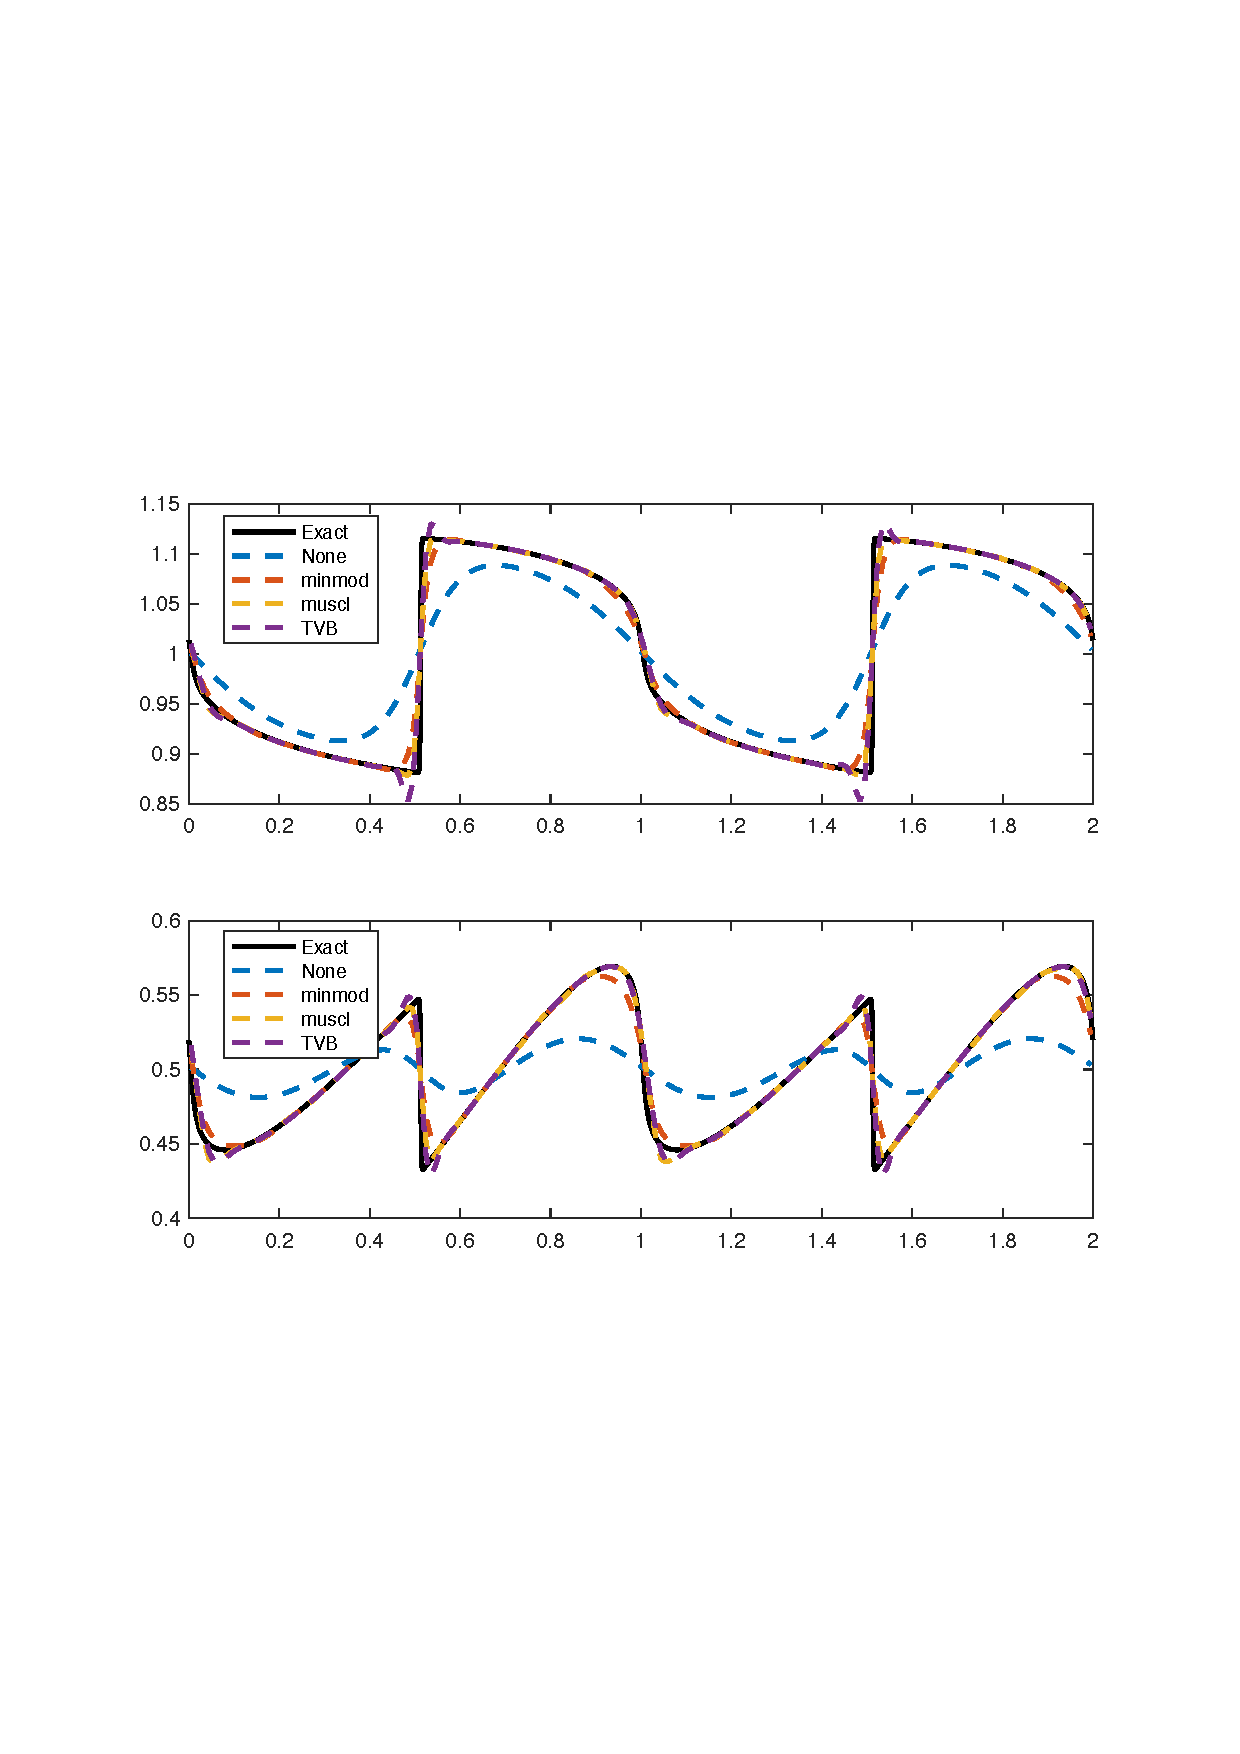
\includegraphics[width=11cm]{2_2_a_IC_3_LF.pdf}
    \caption{LF method errors, 500 cells, IC (7)}
    \label{fig:LF_IC_3}
\end{figure}

\begin{figure}[!htb]
    \centering
    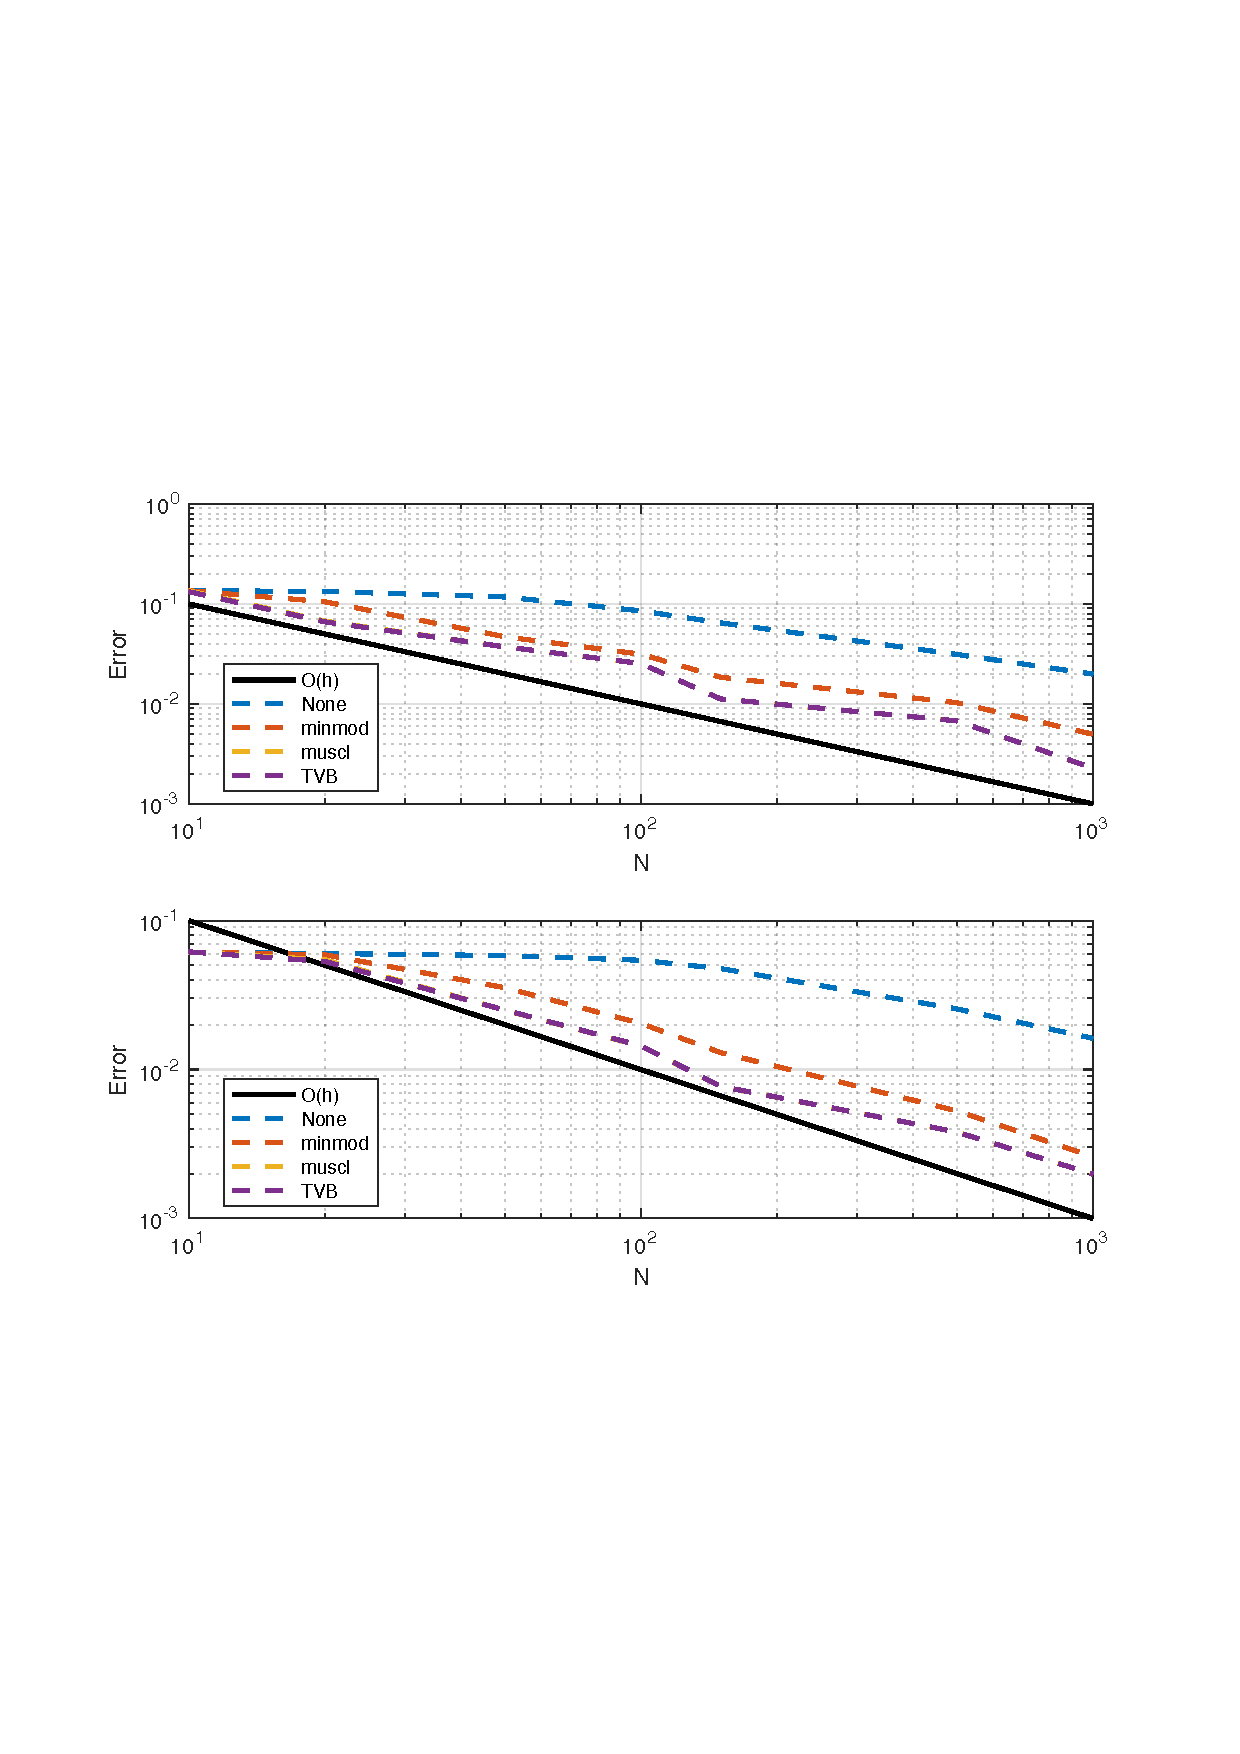
\includegraphics[width=11cm]{2_2_c_IC_3_LF.pdf}
    \caption{LF method at T=2, 500 cells, IC (7)}
    \label{fig:LF_IC_3_error}
\end{figure}

\begin{figure}[!htb]
    \centering
    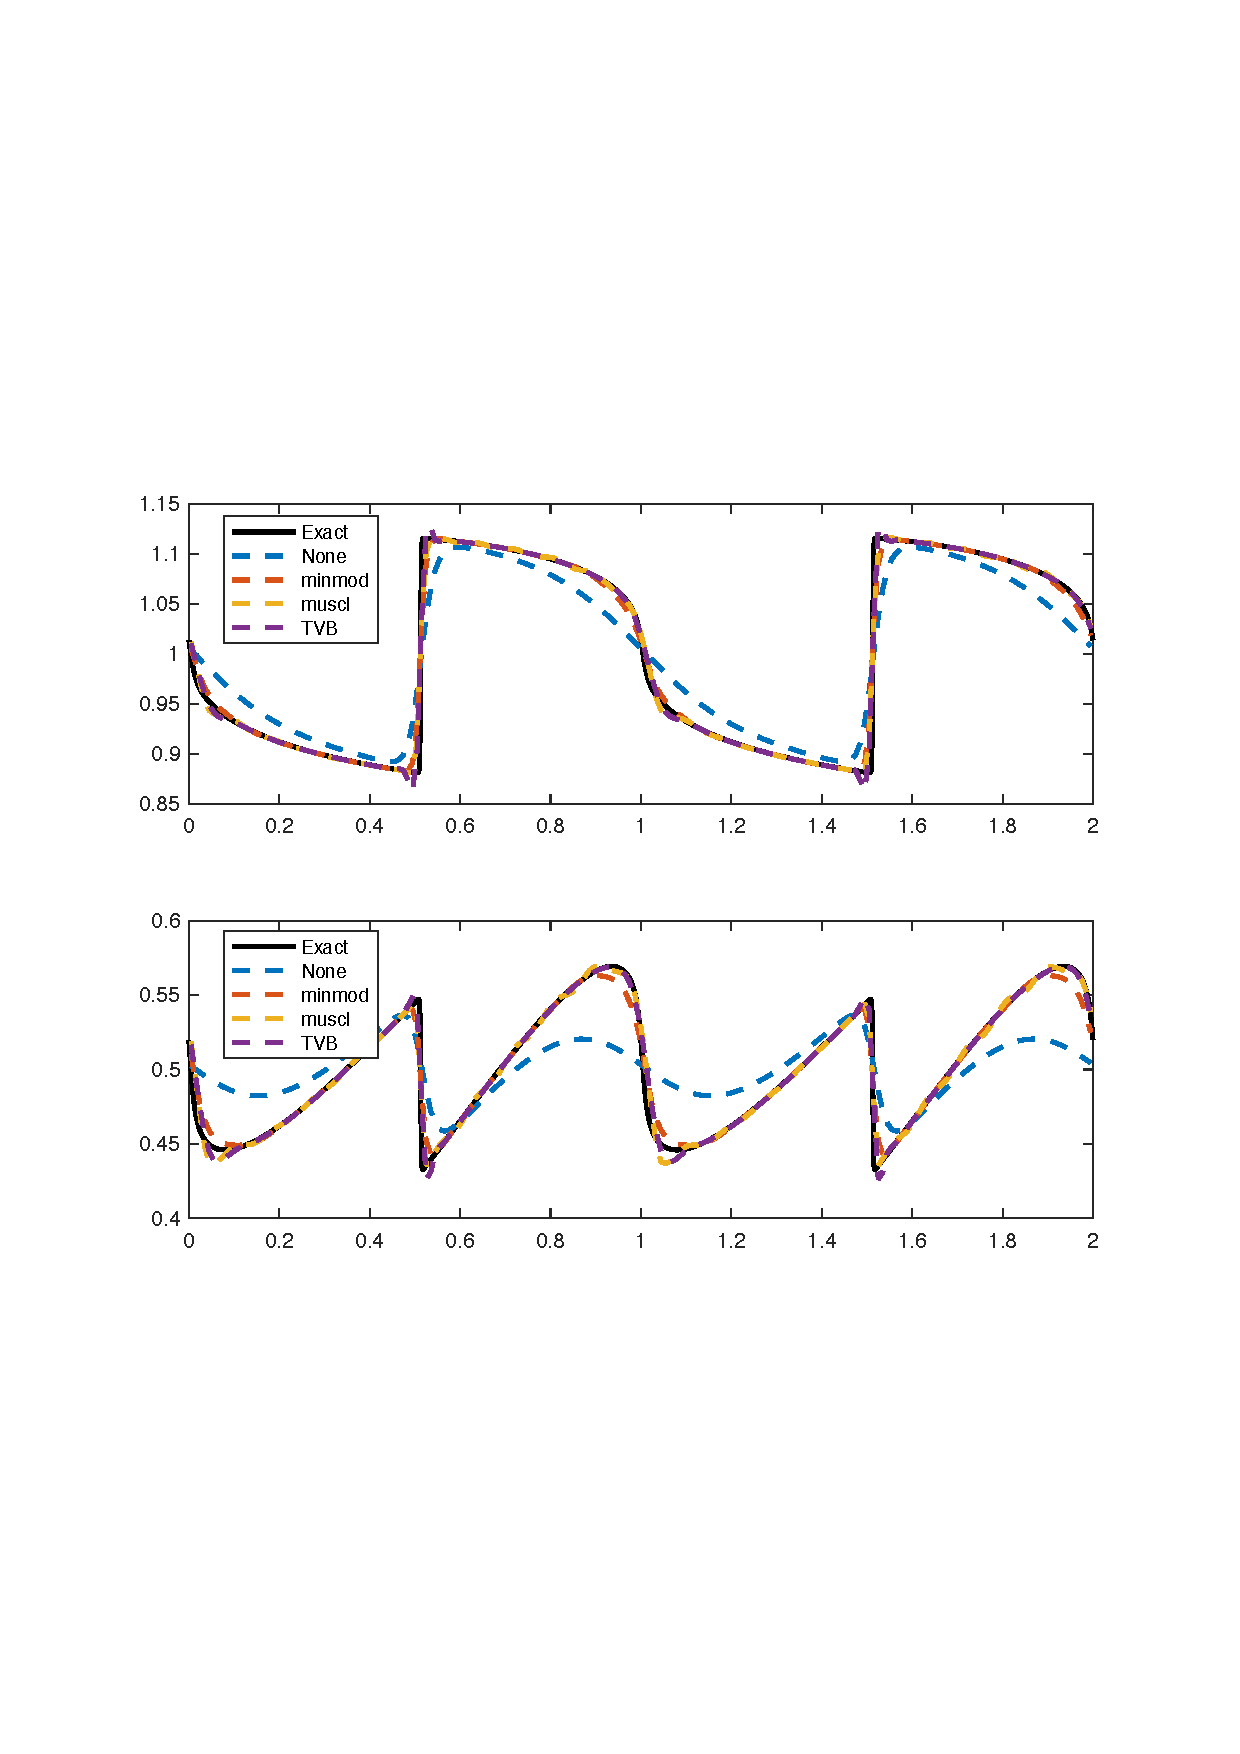
\includegraphics[width=11cm]{2_2_a_IC_3_Roe.pdf}
    \caption{Roe method errors, 500 cells, IC (7)}
    \label{fig:Roe_IC_3}
\end{figure}

\begin{figure}[!htb]
    \centering
    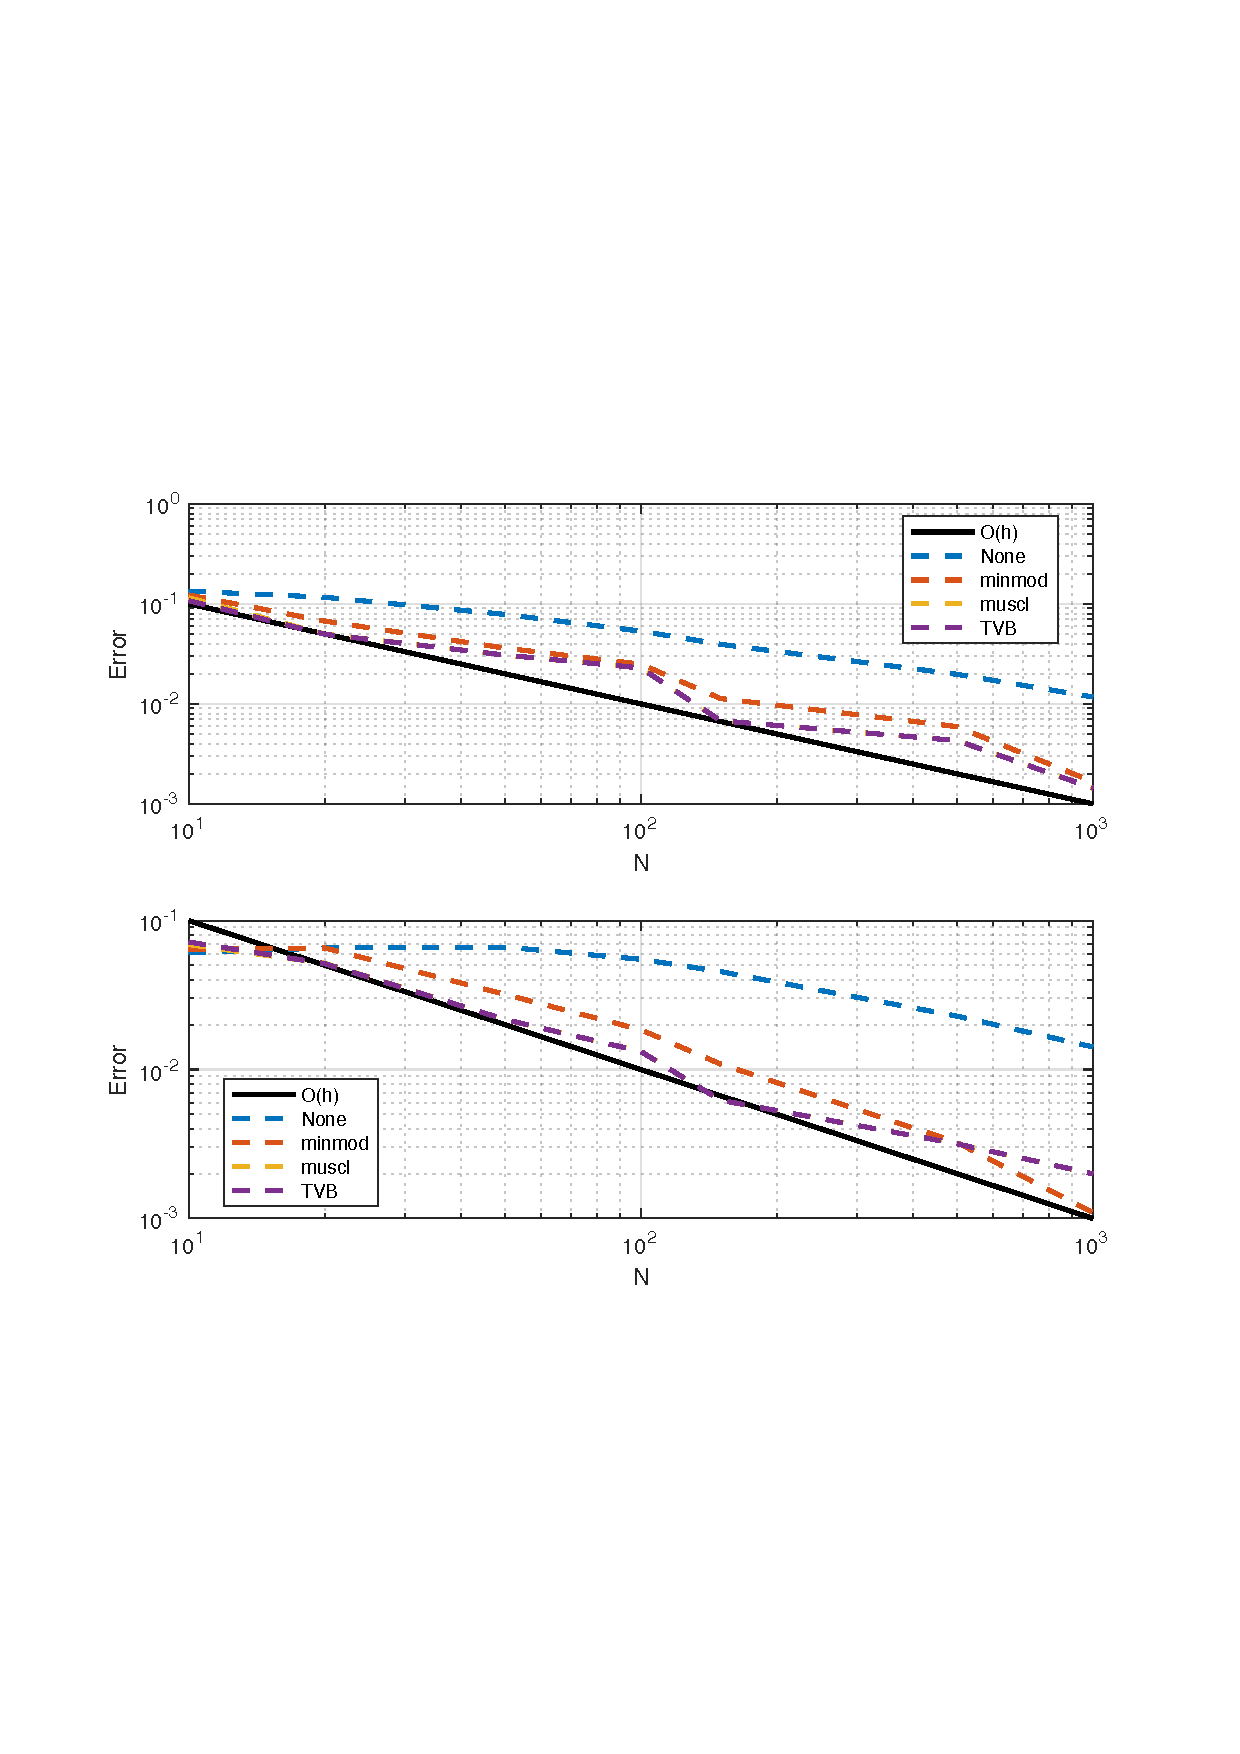
\includegraphics[width=11cm]{2_2_c_IC_3_Roe.pdf}
    \caption{Roe method at T=2, 500 cells, IC (7)}
    \label{fig:Roe_IC_3_error}
\end{figure}

%3_c

\begin{figure}[!htb]
    \centering
    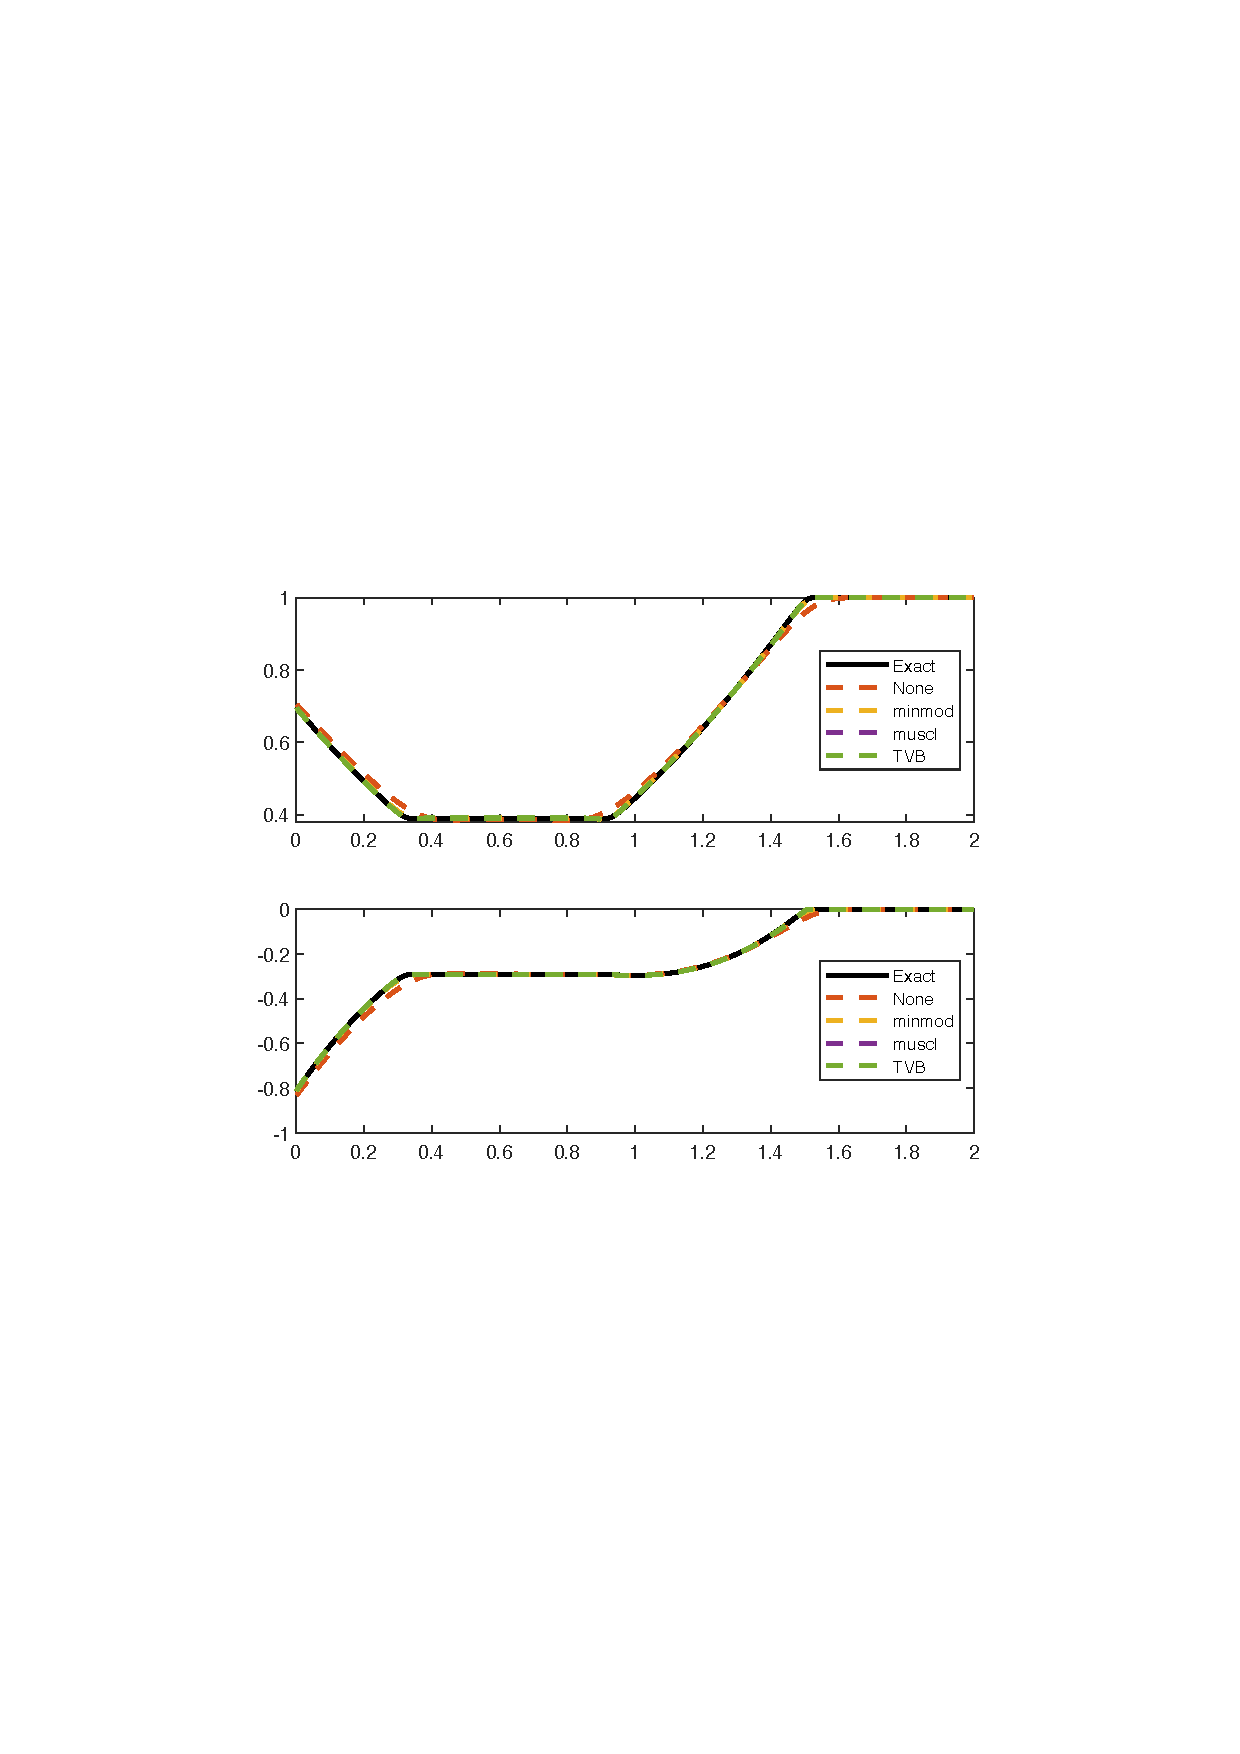
\includegraphics[width=11cm]{2_3_a_LF.pdf}
    \caption{LF method at T=2, 500 cells, IC (8)}
    \label{fig:FL_IC_4}
\end{figure}

\begin{figure}[!htb]
    \centering
    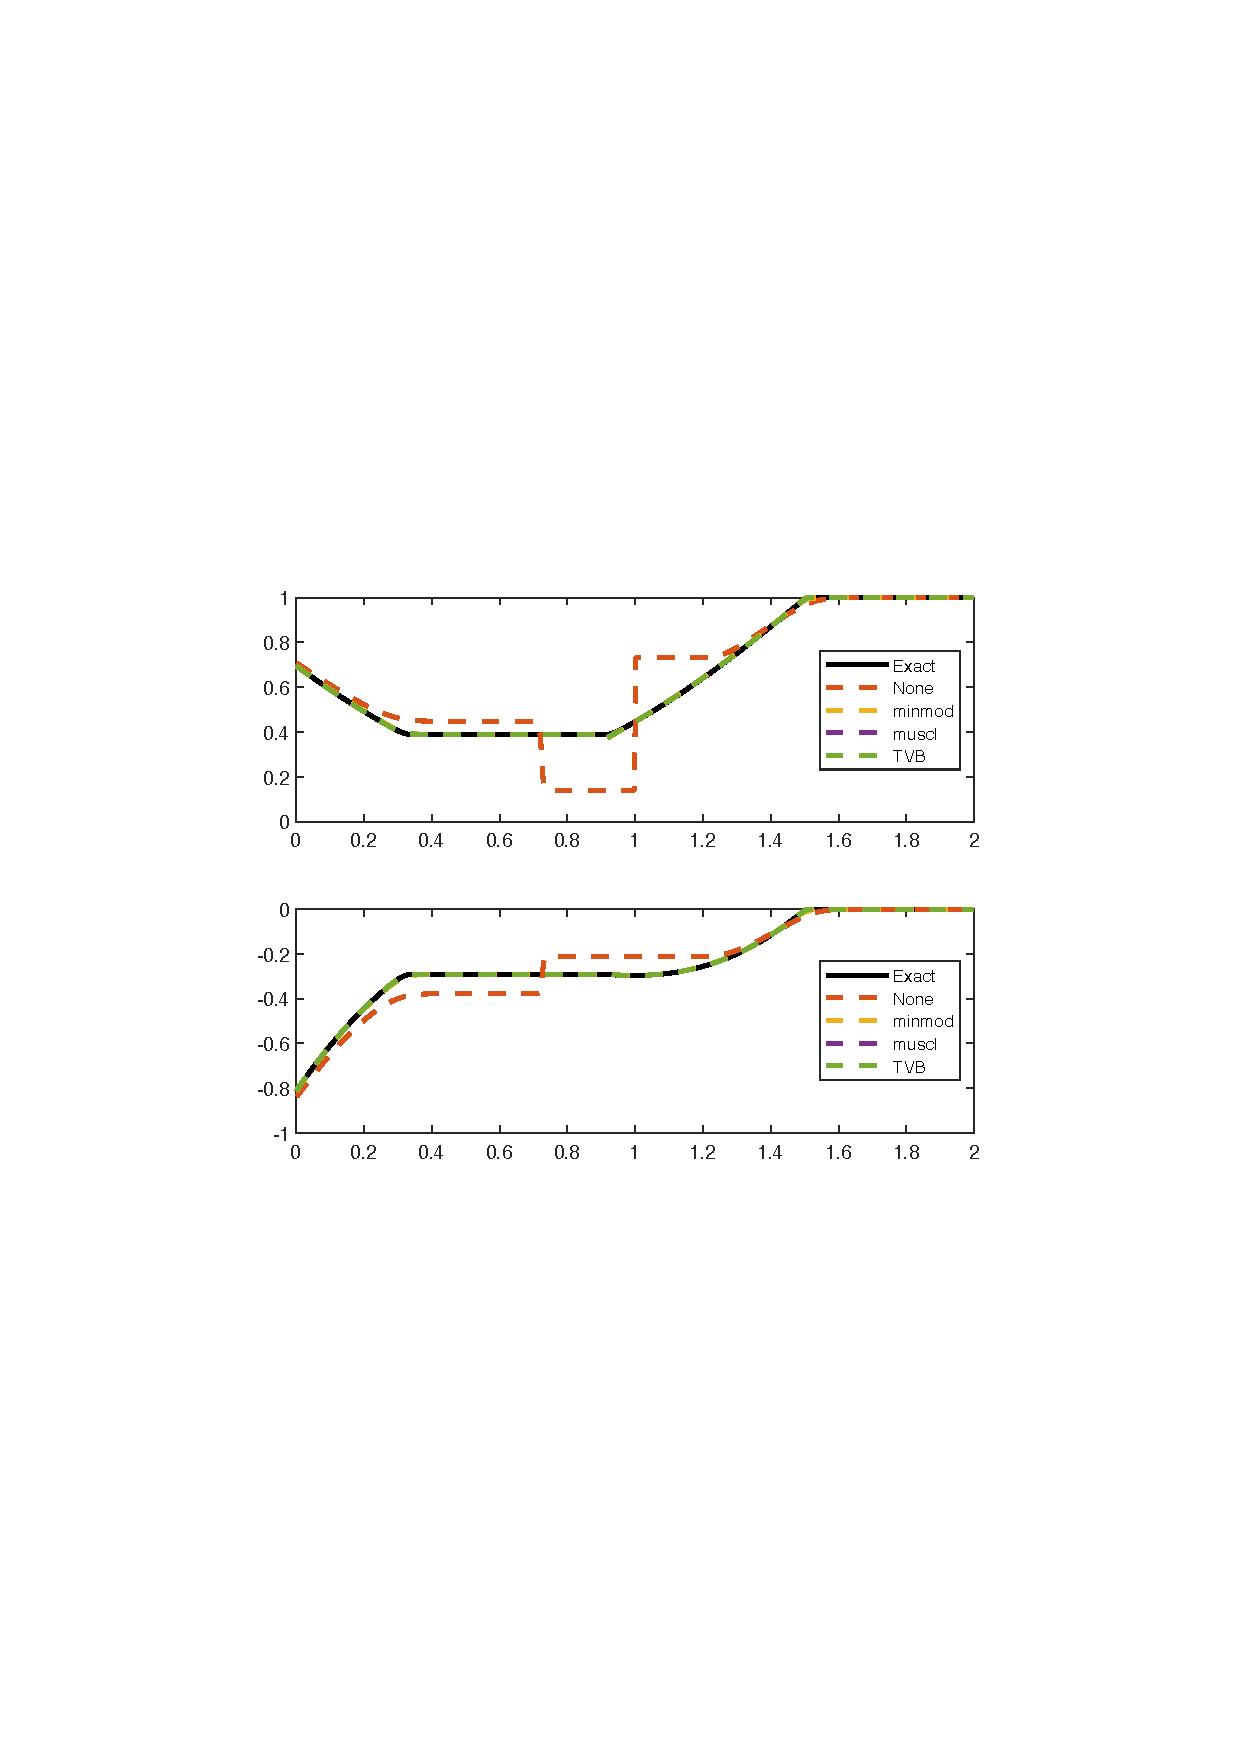
\includegraphics[width=11cm]{2_3_a_Roe.pdf}
    \caption{Roe method at T=2, 500 cells, IC (8)}
    \label{fig:Roe_IC_4}
\end{figure}




%------------------------------------------------------------------------
\afterpage{\blankpage}
\afterpage{\blankpage}
\afterpage{\blankpage}
\afterpage{\blankpage}
\afterpage{\blankpage}
\afterpage{\blankpage}

\newpage
\appendix
%A.1 instead of A.a
\counterwithout*{subsection}{section}
\renewcommand{\thesubsection}{\thesection.\arabic{subsection}}
%Path to .m file
\lstset{inputpath=m}

\section{Utility functions}\label{utility}

\subsection{Applying boundary conditions}\label{BC}
\lstinputlisting{apply_bc.m}

\subsection{Initial conditions}\label{IC}
\lstinputlisting{Initial_conditions.m}

\subsection{Numerical flux}\label{flux}
\lstinputlisting{numerical_flux.m}

\subsection{Evaluating the RHS}\label{rhs}
\lstinputlisting{evalRHS.m}

\subsection{Godunov Flux}\label{G_flux}
\lstinputlisting{GodunovFlux.m}

\subsection{Solver}\label{solver}
\lstinputlisting{solver.m}

\subsection{Error}\label{error}
\lstinputlisting{p_error.m}

\subsection{Compute gradient}\label{gradient}
\lstinputlisting{compute_grad.m}

\subsection{MINMOD}\label{minmod}
\lstinputlisting{MINMOD.m}

\subsection{TVB}\label{tvb}
\lstinputlisting{TVB.m}

\subsection{Slope Limiter}\label{slope}
\lstinputlisting{slope_limiter.m}

\subsection{SSP RK3}\label{ssp}
\lstinputlisting{ssp_rk3.m}

\subsection{Rescaling solution}\label{rescale}
\lstinputlisting{ref_to_current.m}

%------------------------------------------------------------------------
\section{Plotting solutions}\label{plot}

\subsection{LF and Roe with IC (2) and exact solution}\label{plot_IC_1}
\lstinputlisting{p_2_1_b_plots.m}

\subsection{Error of LF and Roe with IC (2)}\label{plot_IC_1_error}
\lstinputlisting{p_2_1_b_errors.m}

\subsection{LF and Roe with IC (6) and (7) and reference solution}\label{plot_IC_2/3}
\lstinputlisting{p_2_2_a.m}

\subsection{Errors of LF and Roe with IC (6) and (7)}\label{plot_IC_2/3_error}
\lstinputlisting{p_2_2_c.m}

\subsection{LF and Roe with IC (8) and reference solution}\label{plot_IC_4}
\lstinputlisting{p_2_3_a.m}






\end{document}
